\section{Project management}
There is a consensus amongst the team members that our adaptation of Scrum has worked well as a project management framework. Combining this with our adaptation of Extreme Programming has led to a very agile and responsive development process. 

\subsection{Preventive measures}
In order to ensure that the productivity continuously peaked, preventative measures were taken early on in the project. One of these measures were that the team instated a monetary penalty for arriving late to meetings or not delivering work on time. The money accumulated from this action was later spent on a team building. The other measure was that one team member was responsible for bringing snacks and making sure the team took regular breaks on the long work sessions on Wednesdays. This arrangement circulated throughout the project. We believe that both of these measures had a good effect on the team, and that they increased the productivity and mood within the team.

\subsection{Working with the customer}
\todo{Dette blir også nevnt under "In-house devices". Kanskje fjerne noe av dette? Fremstår som at vi er litt butthurt. The team tried to have meetings with the customer once a week. This worked well, and the team felt it was a good thing that the customer participated to such an extent. Initially, we had some trouble with the customer not reaching the deadlines that were set in conjunction with the team. This had a negative effect on the team's research in the early stages of the project. 

One of the duties that was not fulfilled by the customer was setting the team in contact with people at SINTEF that might had information on hardware solutions we could use in our project. As this requirement was dropped early on, it did not have a huge effect. However, after sprint five, the team received an e-mail detailing the CoSSMic API, described in section~\ref{sec:cossmicapi}. We think that having this information early on might have made the system easier to integrate and develop in the future. As the information was received so late in the development process, the team and customer agreed on not implementing it Instead, the team should provide documentation on how it could be used in further development.}

\subsection{Changing roles}
\label{sec:unbalancedWorkload}
In the beginning of the project, the team distributed roles with different areas of responsibility, as described in table~\ref{sec:mainresp}. Almost halfway through the project it became clear that the Scrum master at the time, Per Øyvind, also was the team member with the most experience with Android development. 

This resulted in a lot of extra work on the Scrum master, while the deputy project leader only had a few responsibilities. The team reviewed the project roles and the work load distribution, which resulted in a change of roles. The team came to the conclusion that Lars Erik, our now former deputy project leader, was the best fit to be the new Scrum master. After this change, the team's best Android resource could focus entirely on the Android development, and make himself available to help others. The team was very satisfied with this decision, and efficiency and productivity increased after the change in roles.

% Står allerede beskrevet i "Our adaption of Scrum". It was also discussed whether the position `Project leader' actually was necessary, as it conflicted with one of the principles in Scrum. The team decided that the position was necessary as the project leader and Scrum master simply would share the Scrum master's traditional tasks between them. The main difference would be that the project leader would handle the administrative tasks, such as booking rooms for meetings and work sessions, and handle customer relations, while the Scrum master would handle the project administrative tasks. These tasks include moderating of the Scrum meetings, adding tasks to the backlog and Yodiz, and generate burn down charts.

\subsection{Choice of development methods}

The team used Scrum together with Extreme programming. This process and why these were chosen is described in section \ref{sec:scrumDevProcess} and~\ref{sec:adapExtremeProgr}. Although Scrum is a well known development method, a lot of the team members had different expectations to how the framework would be implemented in the project.

\todo{Dette er også beskrevet i "Android development" under "Architectural choices". Flytte noe av dette dit? For det handler egentlig ikke så mye om hva vi syntes om utviklingsmetode. Each team member spent a significant amount of time getting up to speed with the Android platform and the front-end architecture of Android apps. In retrospect, more time should have been spent getting all group members up to date and practicing Android programming together in the beginning of the project. One of the team members had some experience with Android before and ended up spending a lot of time teaching and explaining to the other team members. If this had been organized in a way, for instance by holding a course in the beginning, some of the time spent on this could have been saved. }

\subsection{Underestimation of workload}
A prevalent risk to any project is the failure to acknowledge the cost of tasks in the project and the improper allocation of resources that follows such an error. This can also lead to a false sense of what a team can achieve in a given time frame. 

The team experienced this risk to have the biggest negative impact on our work flow. Even though it did not have a detrimental effect on the sprint end result, it was the most occurring risk, which added up to be very time consuming. The main reason for this issue was the lack of experience with many of the tasks, but also that we initially did not consider who the tasks were assigned to, which turned out to play an important role in the equation. Learning from previous mistakes, the team started looking at previous sprint backlogs to help with the estimation of the tasks.

\subsection{Choice of Scrum tool}
\label{sec:choiceScrumTool}
As the team did not have daily meetings, a good Scrum tool was needed to keep track of progress. Having bad experiences with Scrum tools from previous projects, the team decided to spend some time to research the possible candidates. After Yodiz was chosen, we were confident we had made the best decision, considering all available options. This still might be true, but using Yodiz nonetheless proved to be somewhat frustrating for the team members. An example of an event that caused a lot of frustration in the early stages of the project is given in the subsequent section. Another example is that the burn down charts that Yodiz generated turned out to be useless for documentation. This lead to the team having to do the burn down charts manually. As a matter of fact, a digital Scrum tool is very hard to design in an intuitive fashion. Combined with poor support for simultaneous editing and a lot of down-time for the web-page, the result was a system that causing problems. 

However, Yodiz was the only tool that covered all the requirements set by the team, and despite its obvious flaws, it did its job. Ideally, the team would have liked to have a meeting room with a Scrum board so the use of such an extensive Scrum tool could be avoided altogether. At the end of the project the team started using a Scrum board in the meeting room that was used on our work sessions. This could have been done earlier in the project.

\subsubsection{Improper use of Yodiz}
\label{sec:improperScrum}
Despite the team's efforts to get acquainted with Yodiz a misunderstanding arose, and was not discovered until the end of the second sprint.

The misunderstanding, displayed in figure~\ref{fig:wrongUse}, was that the team
assumed one could add multiple individuals as responsible on a particular task,
while Yodiz' functionality only assigned the time spent to the individual that was assigned as owner of the task.

As a result, it appeared as if only singular individuals performed the tasks,
even though the entire team in reality was participating, which was also
reflected in the burn down charts and the generated Gantt diagram. 

To sort out this issue, we went through old meeting reports and time sheets
to figure out which members of the team that had actually participated on the
particular task, and added new tasks and the time spent to the members that at
the time had not recorded this information.%, as shown in figure~\ref{fig:addsTasks}.
 This issue was unfortunate, but not insurmountable, and also not a critical
issue for the overall progress of the project.

\begin{figure}[H]
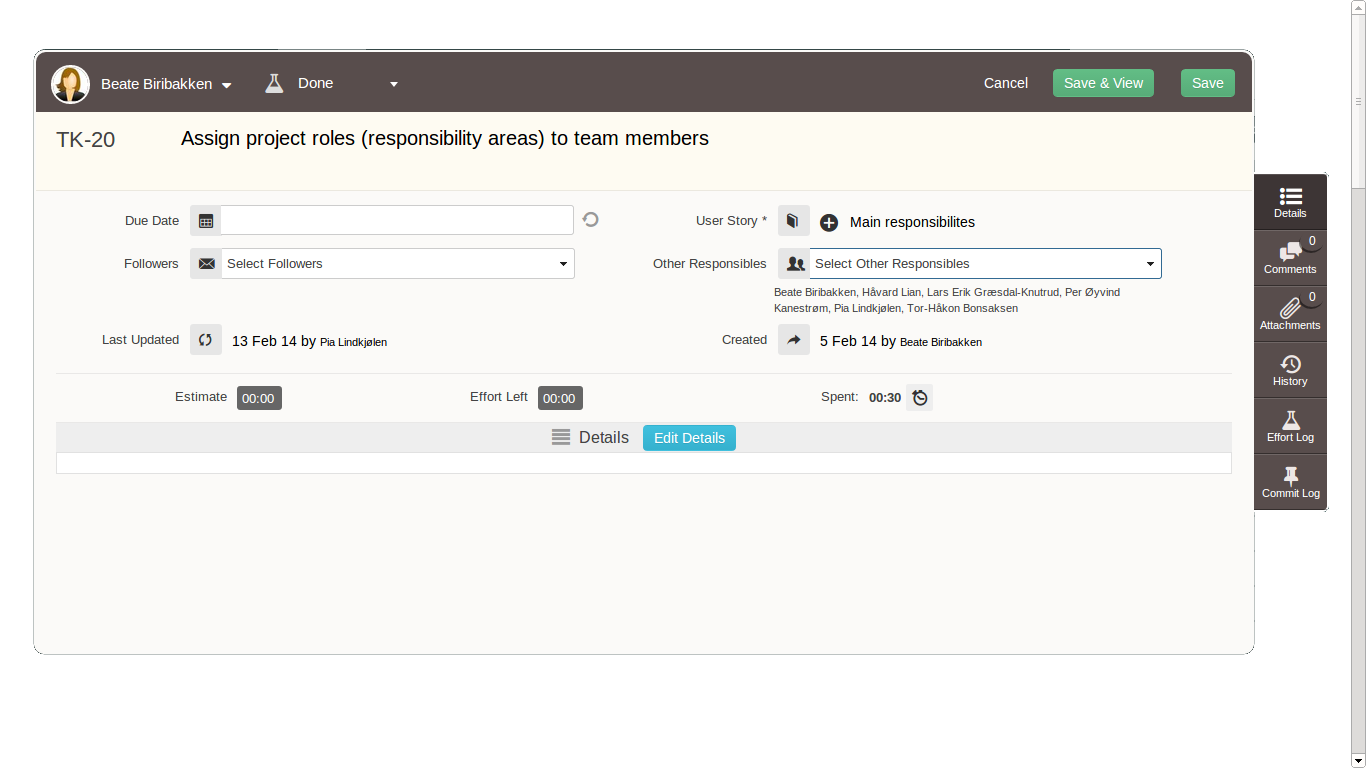
\includegraphics[width=\textwidth, clip, trim=1cm 2cm 4cm 1cm]{ch/retrospect/fig/wrongUse.png}
\caption{Example screenshot to illustrate improper use of Yodiz.}
\label{fig:wrongUse}
\end{figure}
